\chapter{Conclusion and Future Scope}
\label{conclusion}

\section{Sci-Genie: Technical Debts and Shortcomings}
main points : 
\begin{itemize}
    \item Incomplte data as only 25-30K papers are currently correlated
    \item Parsing is heuristic and can be improved several folds using more intelligently methods using ML. The current structure used to index documents can provide context around CS research at search time. For other domains much more grannular 
    \item Sci-Genie doesn't parse PDF and uses Latex which allows for much grannular access to the parsed strcuture and intercompilability to HTML. A lot research in other fields is present in PDF and Sci-Genie doesn't have PDF mining capabilities. 
    \item Lucene based indexes are not the best choices when 
\end{itemize}

\section{Future Research Scope}
\label{conclusion:future-scope}
\subsection{Grannular Table Type Classification}
\label{conclusion:future-scope:type-class}

The table types defined by \cite{kim2012scientific} are general purpose descriptions which can apply to various domains. Although they are quite useful, tables in recent CS literature have more grannular sub-classifications. For example a "Statistics Table" could be describing a Dataset for Machine Learning experiments. The tables which may seem as Experiments Results can also be describing an Ablation Study conducted on a ML model. Due to a very nuanced distinction between a lot of these tables, The task of machine learning to classify table types needs more grannular sub-types within the classes defined by \cite{kim2012scientific}. 

Multiple grannular table types such as Ablation Study, Dataset Descriptions, can also be further described based on the field of research the tables belong to. The interface shown in Figure \ref{figure17}, was developed to annotated tables from scientific research. This interface can be extended for many fields outside CS for the effort of curation and benchmarking of ML models for indentification of various types of tables from different avenues of research. 

\subsection{Discovering Related Tables}
\begin{figure}[h]
    \centering
    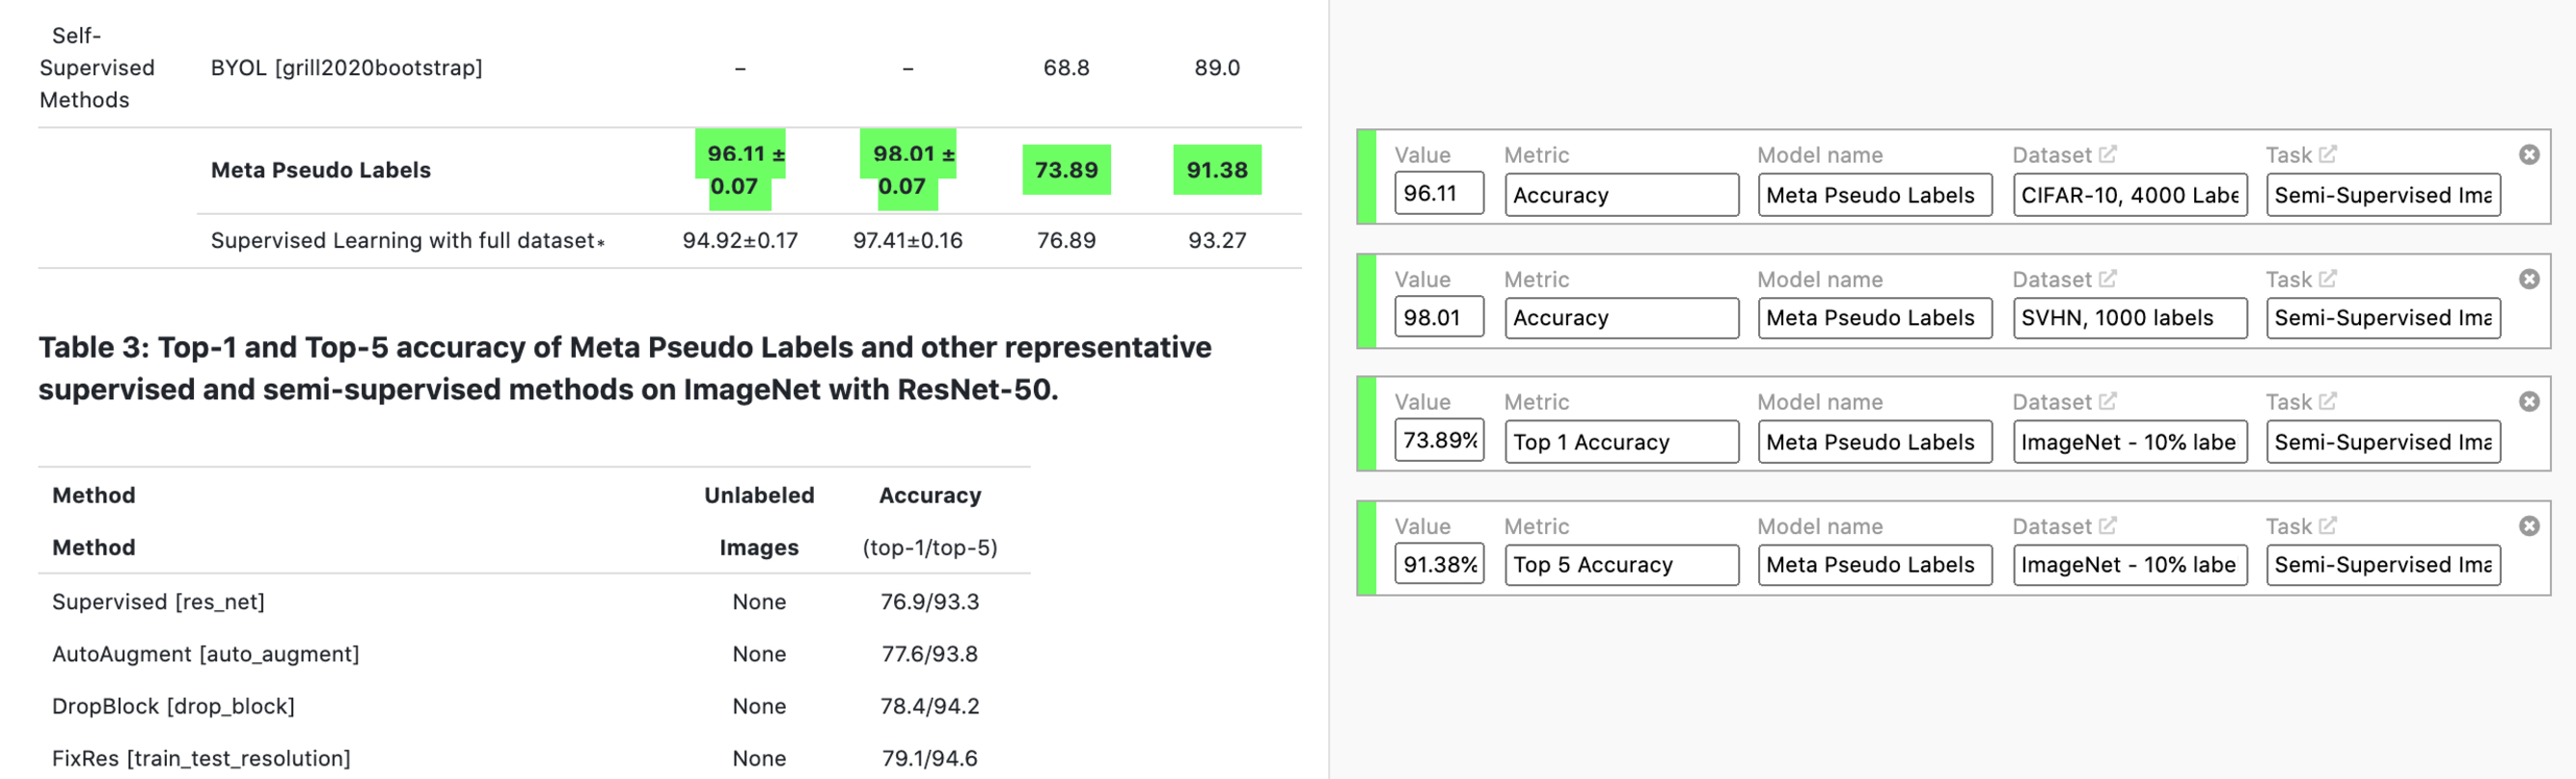
\includegraphics[width=\maxwidth{\textwidth}]{src/images/pwc-table-exp.pdf}
    \caption{ Viewing Tables From SOTA benchmarks }
    \label{figure\arabic{figurecounter}}
\end{figure}
\refstepcounter{figurecounter}
Organisations such as PapersWithCode(PwC) have developed tools to collate information about SOTA ML methods from papers on ArXiv. PwC after parsing these tables either correlate some metrics manually and some intelligently via the use of libraries like Axcell\footnote{https://github.com/paperswithcode/axcell}. This task can become more intelligent and automated where ML models can be developed to correlated tables from research documents from diverse domains outside CS. Discovering related tables using a citation graph and machine learning techniques can be a great direction for future research. 

\subsection{Scientific Research Document Parsing For Search Context}
Google search pivoted to ranking results for search using BERT.\footnote{https://blog.google/products/search/search-language-understanding-bert/} since 2019. This trend of using language models to help rank search results has lead to creation of opensource tools\footnote{https://github.com/deepset-ai/haystack} over off the shelf search engines like Elasticsearch. Although the models help improve search ranking, more nuanced search context result information is yet not accessible via academic research search engines. 

Intelligent parsing maybe one part of the solution. Sci-Genie are uses domain sepecific content parser which is heuristically derived (Chapter \ref{sci-genie-core:scraping:frag-to-rs}) to help bring context relevant information in search results. This parser may not be extensible to various other domains or document types.

\cite{kashyap2020sciwing}, introduced deep learning based techniques for scientific document parsing. But parsing can also be posed a domain specific problem where each domain generally follows a different parse structure. For example, recent papers in Machine Learning explicitly discuss datasets as a section in the paper.

Every domain's specific nuances requires more intelligent systems that can learn to identify such traits on their own. Intelligent techniques of parsing and indexing data to provide sufficient context to the users seems a rich direction of research in the future.

\section{Conclusion}
The fast rate of growth in technological progress will dramatically increase the growth in the volume of research in the future. Figure \ref{figure1}, is the best proof of that insight. The growing volume of research would also require more nuanced search tools which can help surface enough context around search terms and futher aid the researcher when reading research. This dissertation described a search engine and browser app based prototype solution to help remediate this problem. This dissertation covered the formulation of different aspects of the search engine and the ML models powering its table of comparison filtering algorithm. 

In summary, the proposed solutions in this dissertation try to remediate the problem of growth in the volume of research by aiding the researcher with more context based information when searching for research and reading research.